\documentclass[english]{article}
\usepackage[english]{babel} 
\usepackage[T1]{fontenc}
\usepackage[utf8x]{inputenc}
\usepackage{float}
\usepackage{graphicx}

\makeatletter
\usepackage[a4paper,top=2cm,bottom=2cm,left=2cm,right=2cm]{geometry}
\usepackage{enumitem}
\usepackage{subfig}
\usepackage{amsthm}
\usepackage{amsmath}
\usepackage{epstopdf}
\usepackage{fancyhdr}
\usepackage{booktabs,array}

\hyphenation{english}
\makeatother

\usepackage{babel}


\usepackage{listings}
\usepackage{xcolor} % for setting colors

% set the default code style
\lstset{
    frame=tb, % draw a frame at the top and bottom of the code block
    tabsize=4, % tab space width
    showstringspaces=false, % don't mark spaces in strings
    numbers=left, % display line numbers on the left
    commentstyle=\color{gray}, % comment color
    keywordstyle=\color{blue}, % keyword color
    stringstyle=\color{red} % string color
}


\begin{document}
\begin{titlepage}

	\begin{center}
		\begin{Large} \textbf{UNIVERSITY OF PADOVA} \\
		\end{Large} \vspace{1cm}
		\vspace{3cm}
		\begin{Large} Embedded Real--Time Control \end{Large}
		\par\end{center}

	\begin{center}
		\begin{Large}Laboratory report\\
		\end{Large}
		\par\end{center}

	\begin{center}
		\vspace{2cm}
		\begin{figure}[!htb]
			\centering 
\includegraphics[width=8cm]{figures/unipd-logo.png}\\

		\end{figure}

		\par\end{center}

	\begin{center}
		\vspace{2cm}
		\begin{Large} 
                Alireza - (ID) \\
                Max - (ID) \\
                Pouria - (ID) \\
                Parsa Majidi - (2080216)  \\
		\end{Large} \vspace{2cm}
		\begin{Large} Academic Year 2022-2023 \end{Large}
		\par\end{center}

\end{titlepage}

\tableofcontents
\newpage

\section{Laboratory 1: I2C and Interrupt}

In this lab ....

\subsection{Description}

Lorem ipsum dolor sit amet, consectetur adipisci elit, sed eiusmod tempor incidunt ut labore et dolore magna aliqua. Ut enim ad minim veniam, quis nostrum exercitationem ullam corporis suscipit laboriosam, nisi ut aliquid ex ea commodi consequatur.

\begin{figure}[!h]
	\centering
	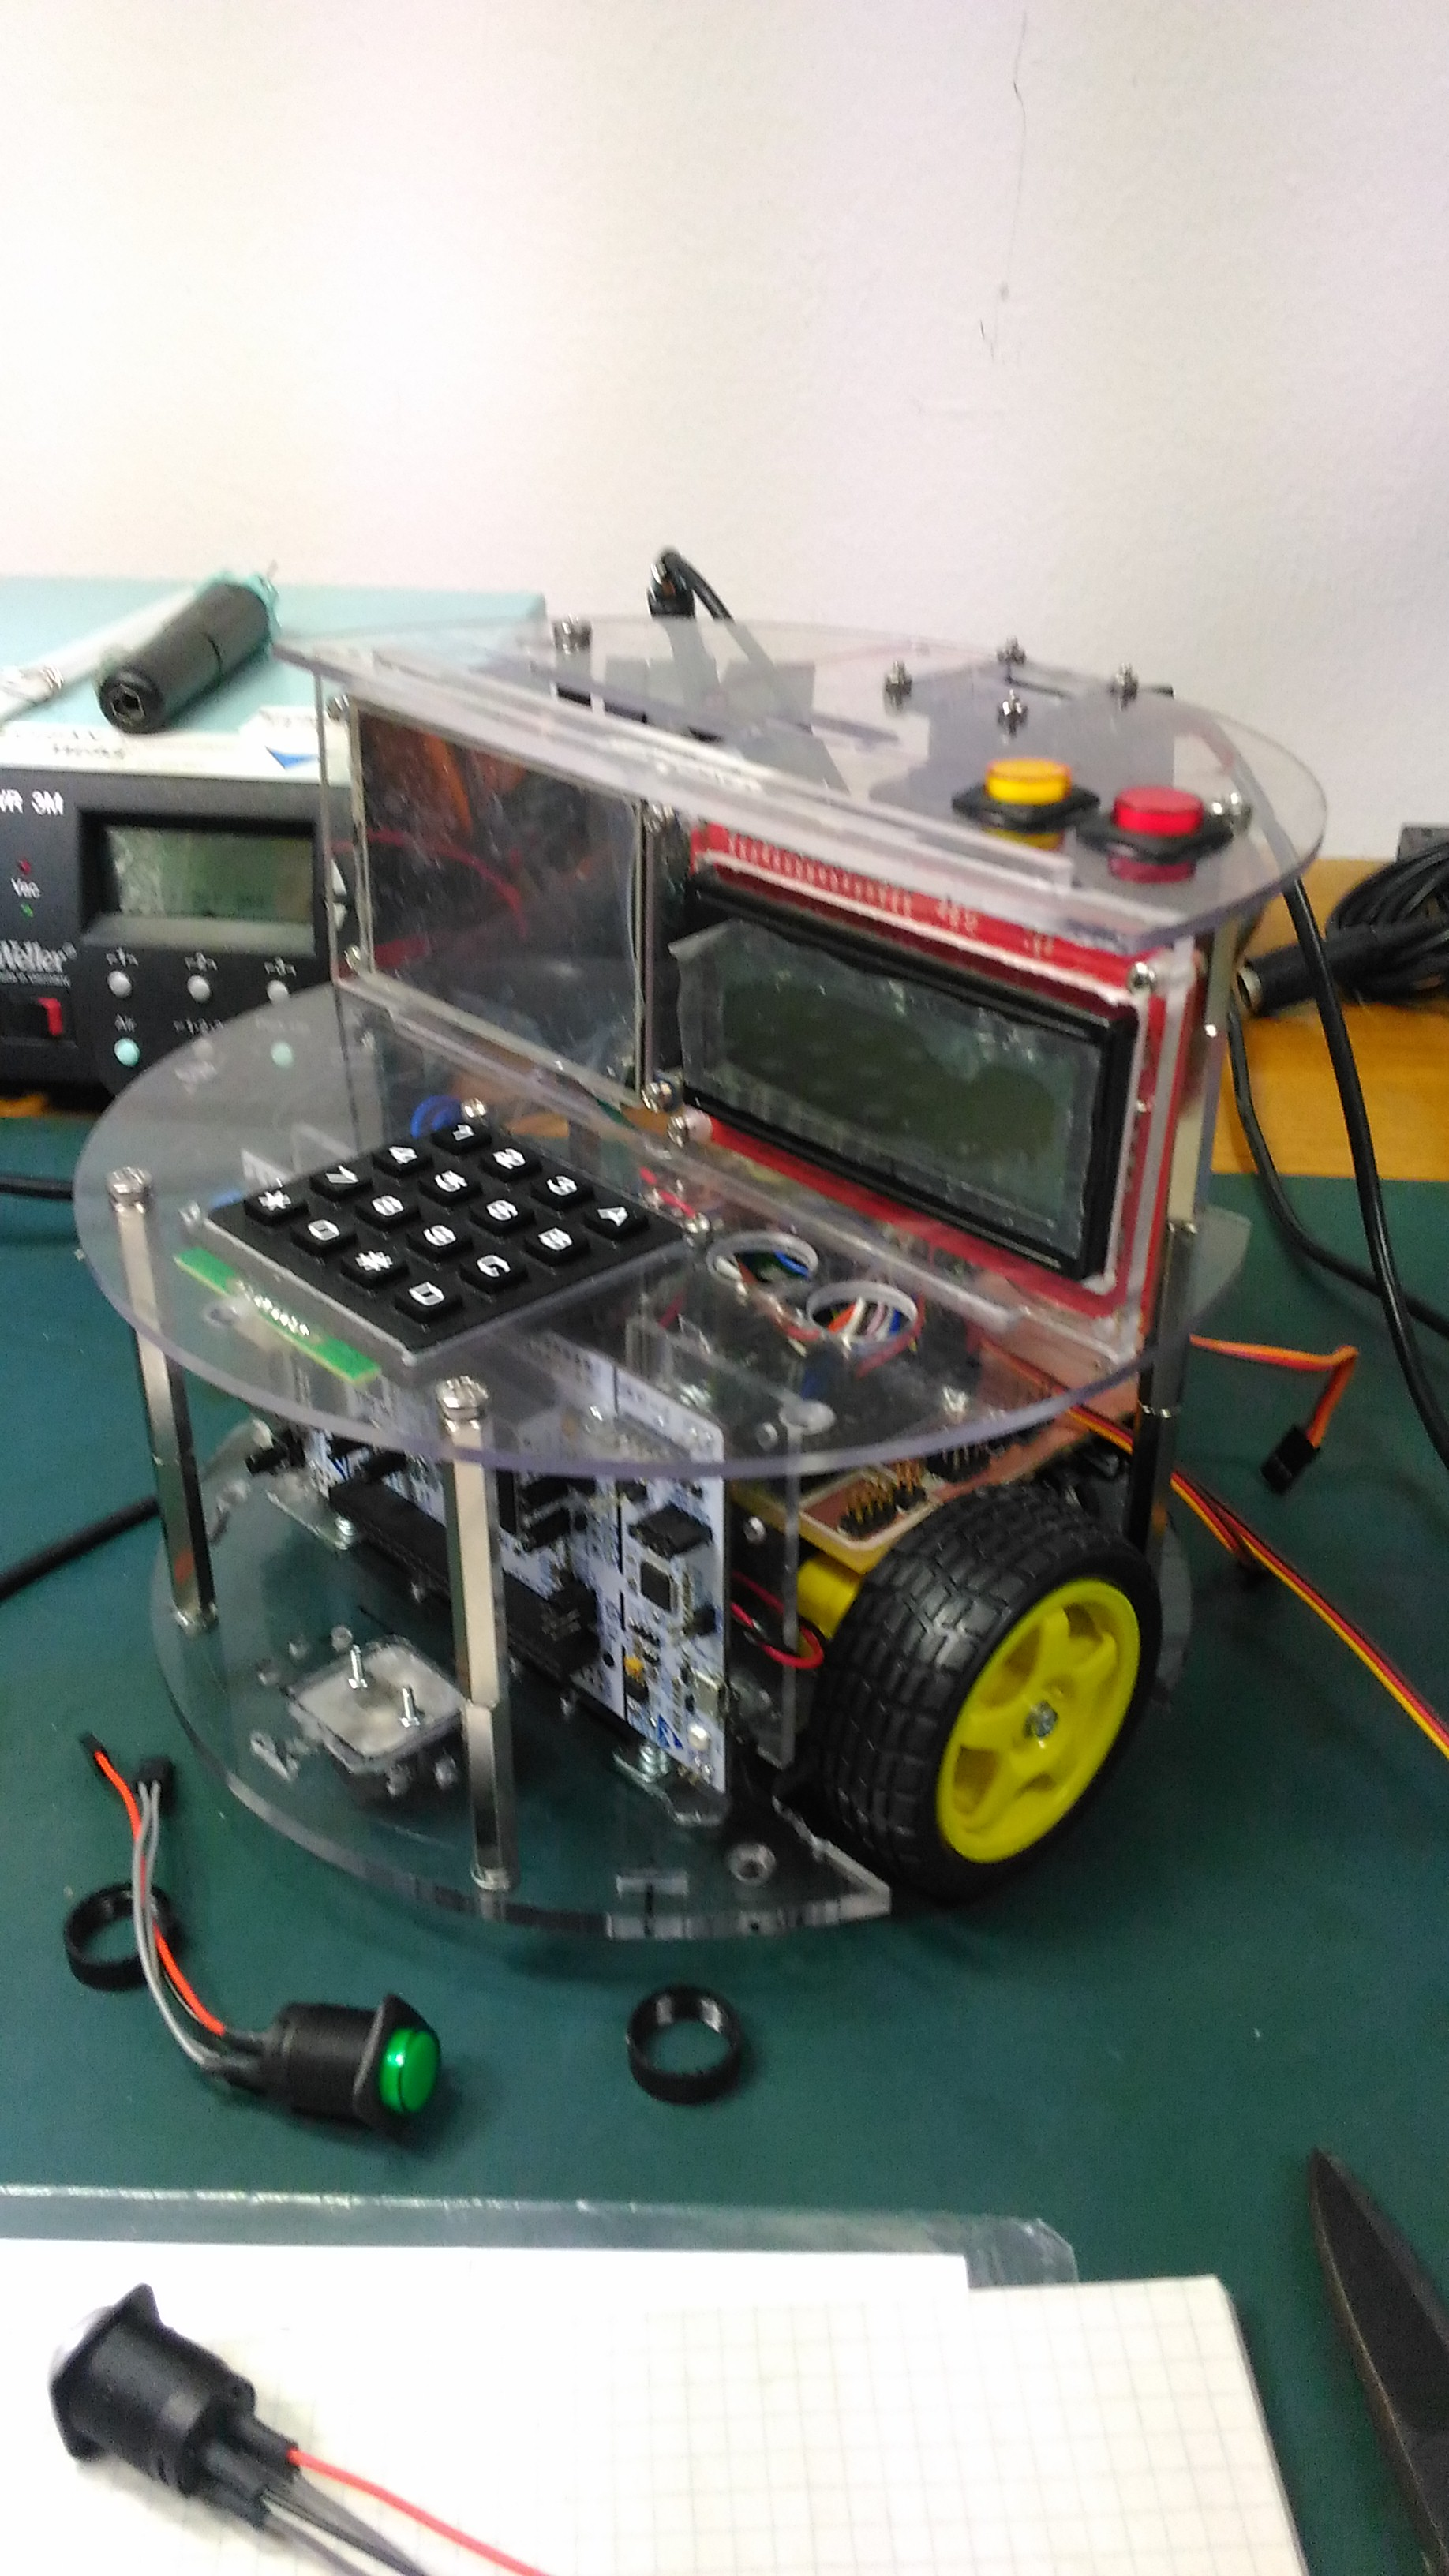
\includegraphics[width=0.4\textwidth]{figures/turtlebot_1.jpg}
	\caption{The TurtleBot}
	\label{fig:turtlebot}
\end{figure}

In Figure~\ref{fig:turtlebot} ...

%\begin{figure}[!ht]
%	\centering
%	\subfloat[The TurtleBot 1 ]
	%{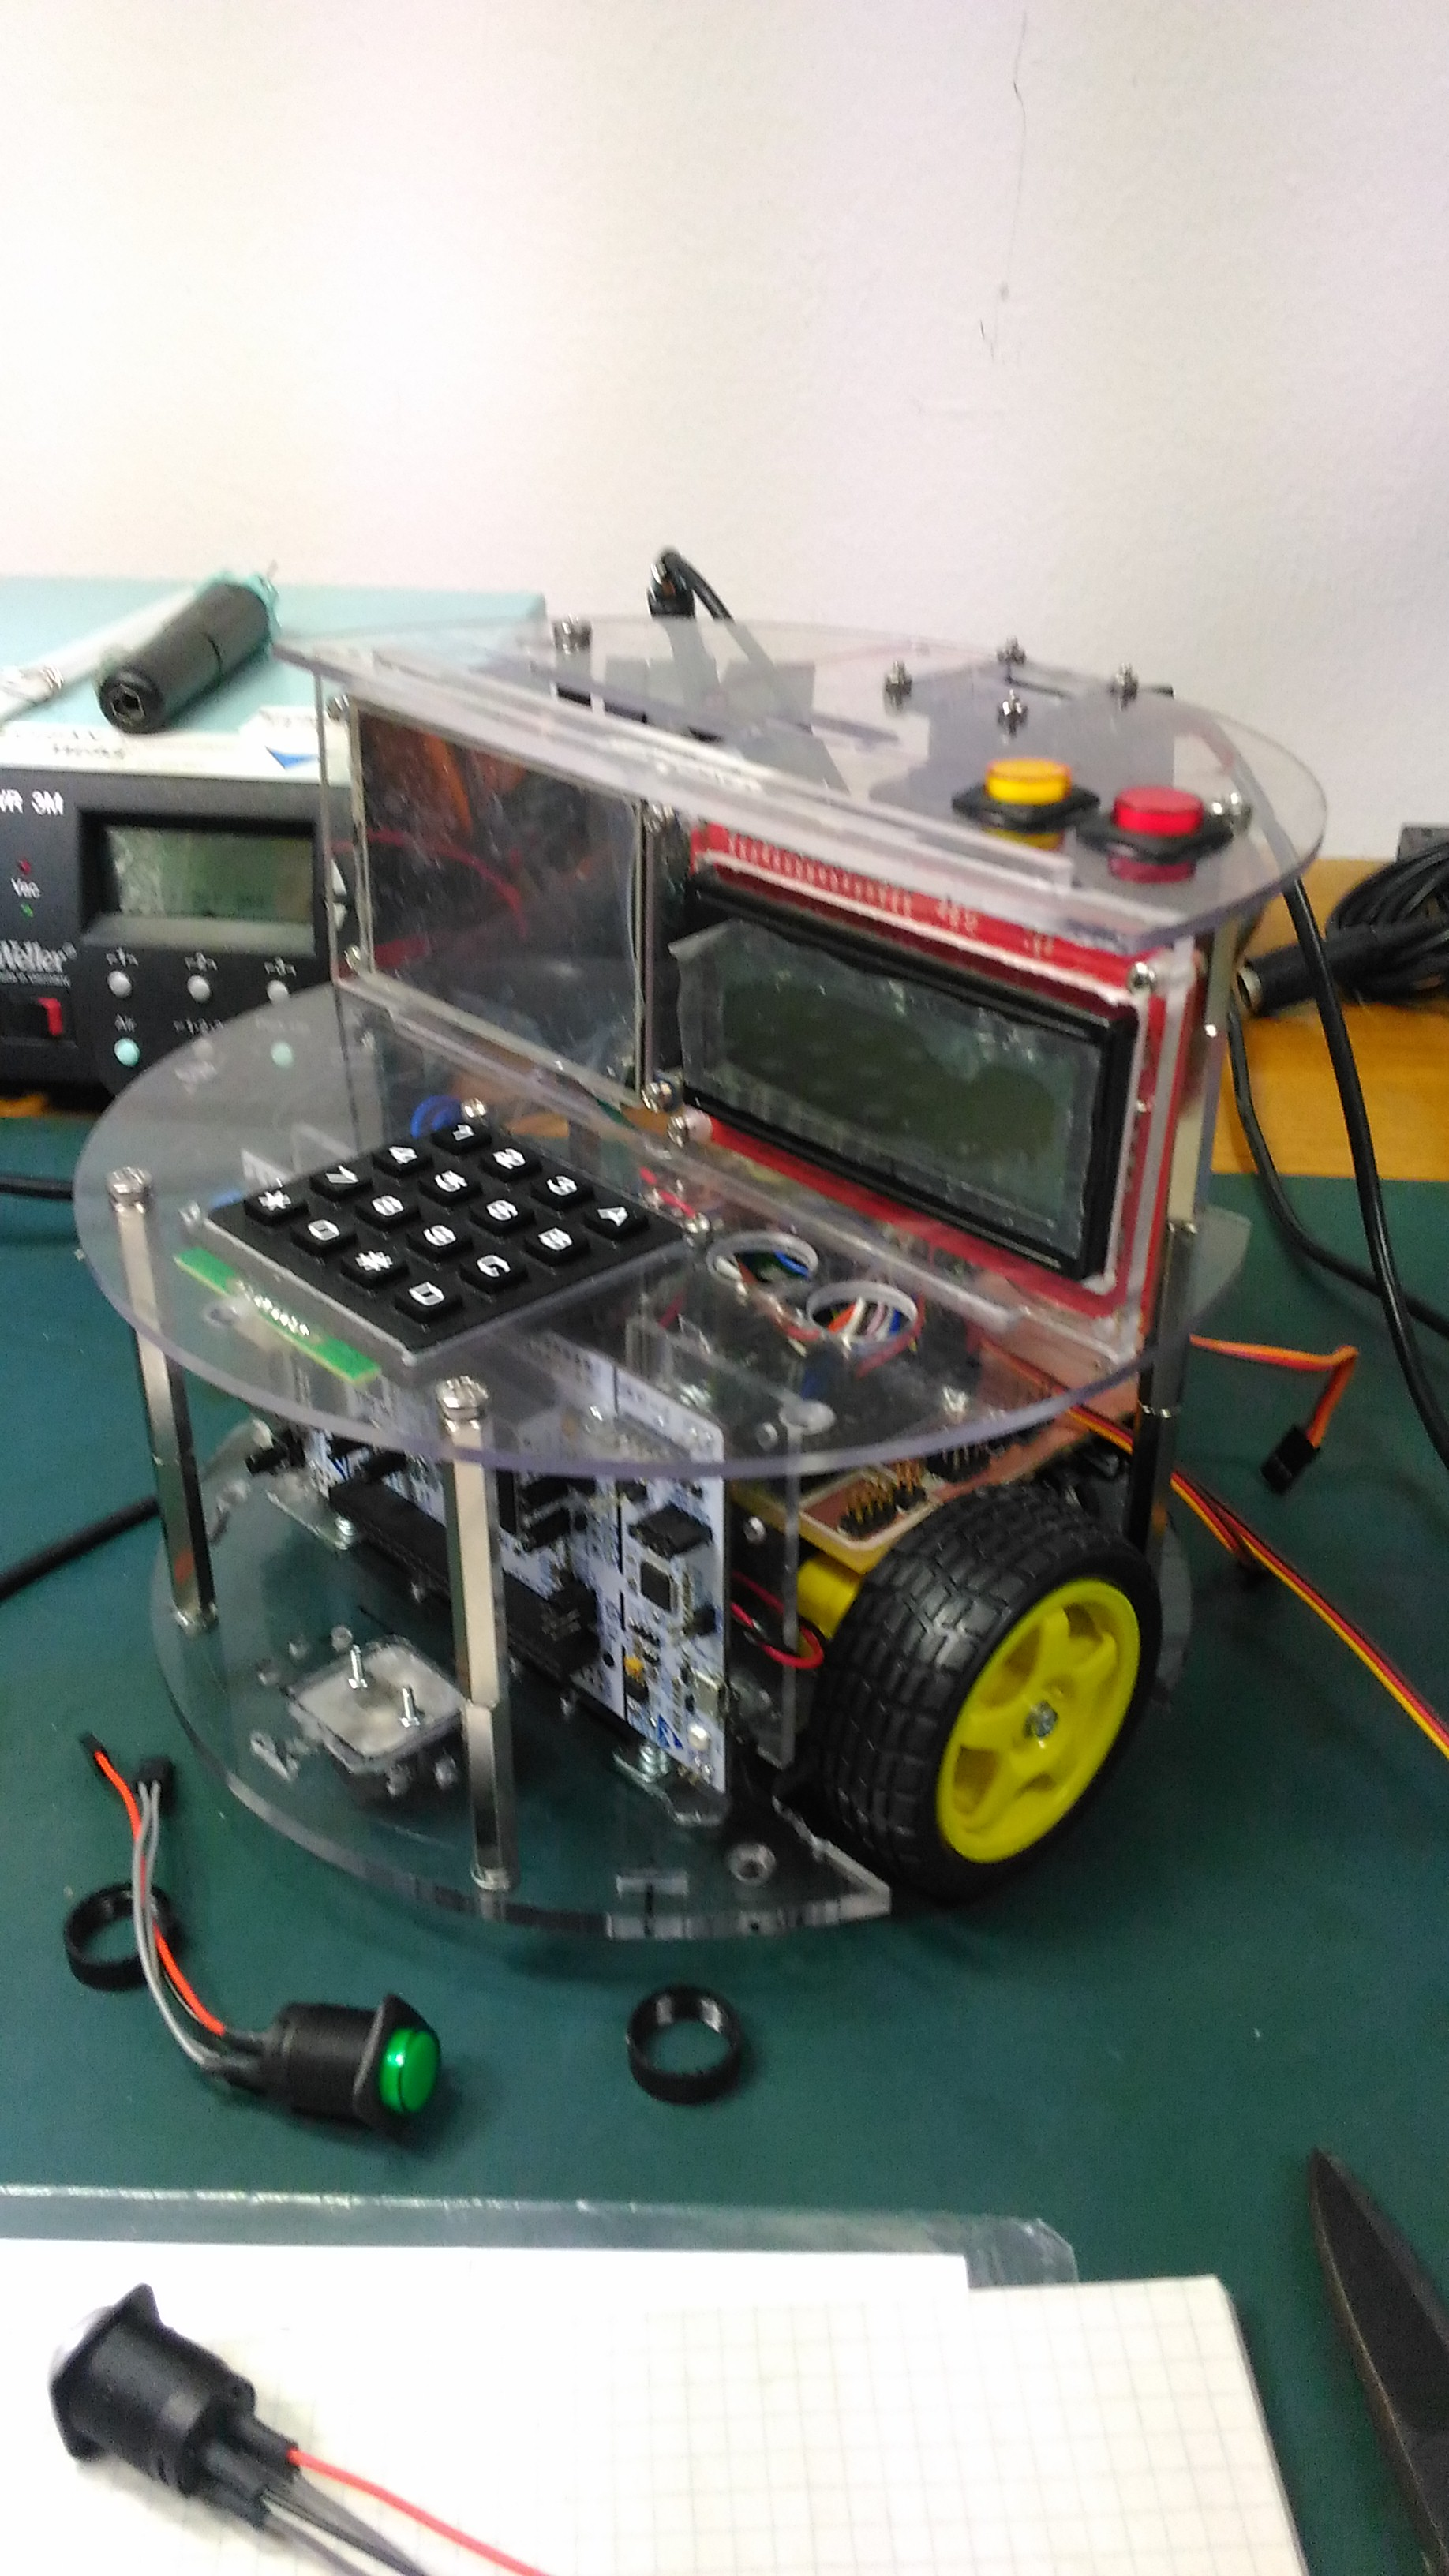
\includegraphics[width=0.3\textwidth,height=0.45\textwidth]{figures/turtlebot_1.jpg}
%		\label{fig:tbot1}}
%	\subfloat[The TurtleBot 2]
%	{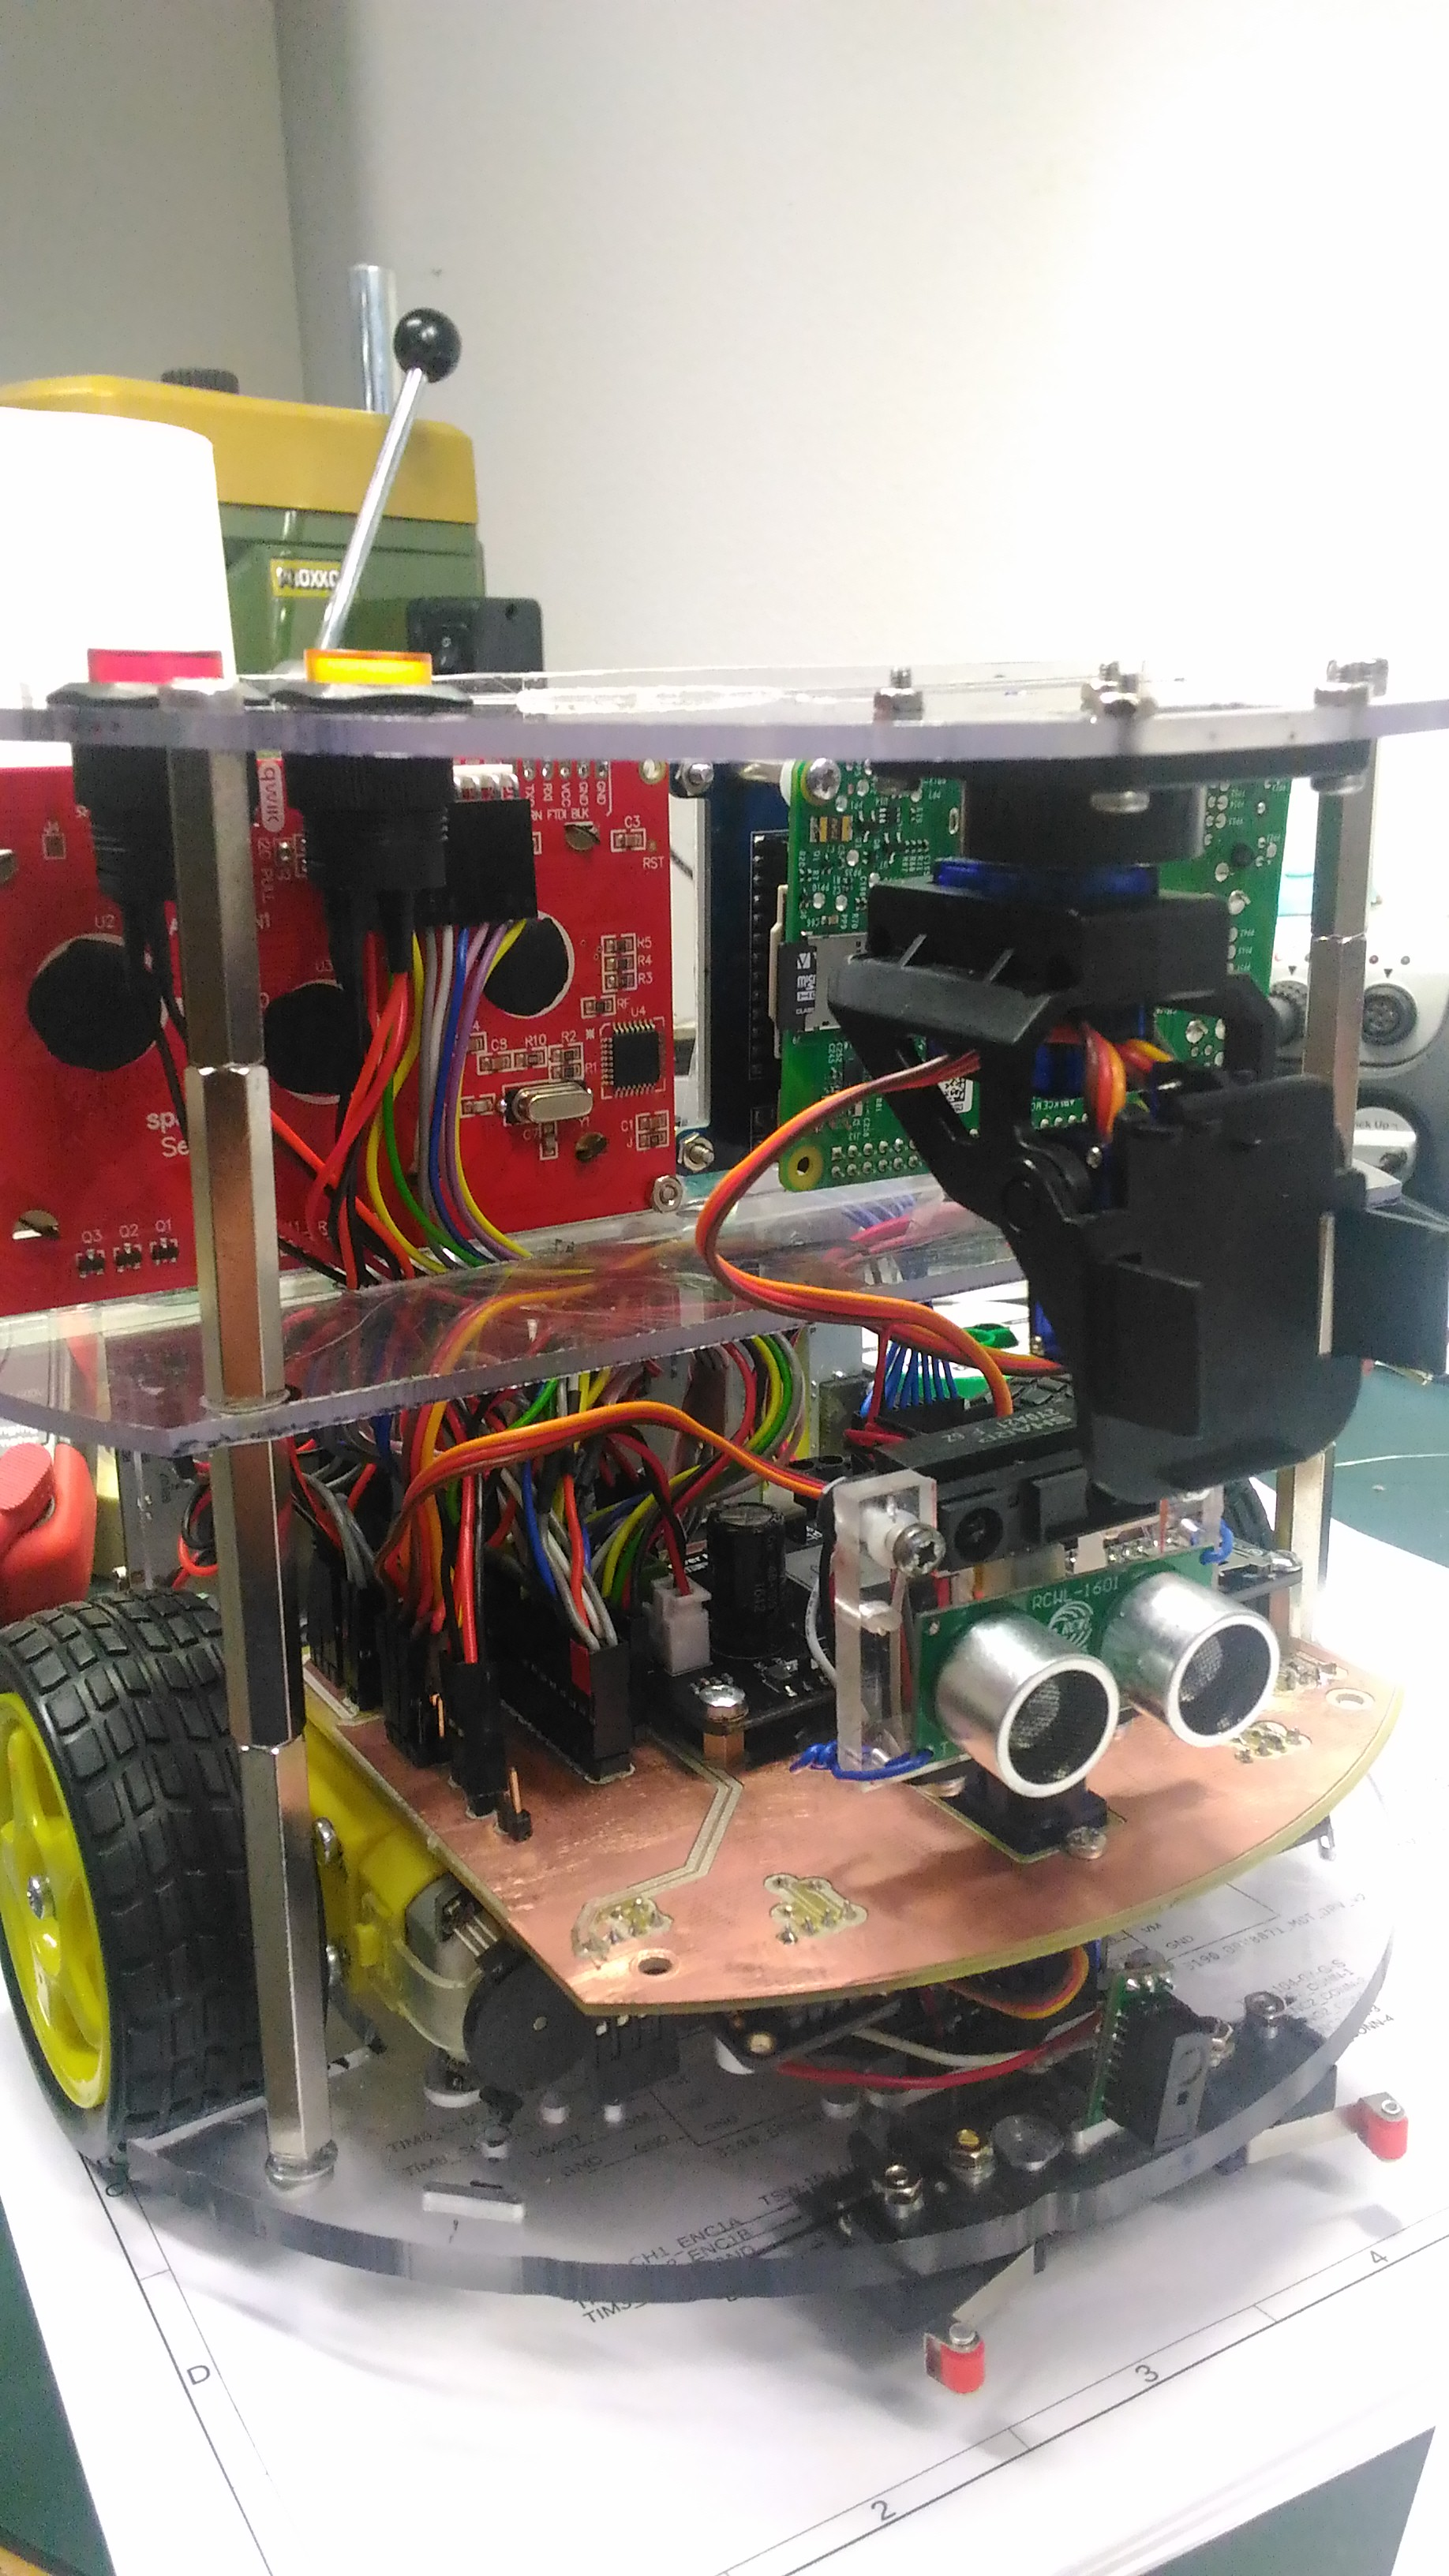
\includegraphics[width=0.3\textwidth,height=0.5\textwidth]{figures/turtlebot_2.jpg}
%		\label{fig:tbot2}}
%	\caption{The TurtleBot}
%\end{figure}

\subsection{STM32IDE}

Lorem ipsum dolor sit amet, consectetur adipisci elit, sed eiusmod tempor incidunt ut labore et dolore magna aliqua. Ut enim ad minim veniam, quis nostrum exercitationem ullam corporis suscipit laboriosam, nisi ut aliquid ex ea commodi consequatur.

\subsection{Sensors}
\newpage
\subsection{Exercise 1:}
\subsubsection{Description}
In this exercise we are asked to write an ISR that recognize and correctly handles the keypad interrupts. We properly implemented the void HAL\_GPIO\_EXTI\_Callback(uint16\_t pin) function, which is used in conjunction with the EXTI (External Interrupt) peripheral to handle interrupts generated by GPIO pins. Then we printed which interrupt has
been triggered i.e. the pin. To be able to receive another interrupt from the keypad, we read
the registers REG\_KEY\_DATA\_1 and REG\_KEY\_DATA\_2 inside the ISR.
\subsubsection{Code}
\begin{lstlisting}[language=C, caption={Interrupt Callback}]
void HAL_GPIO_EXTI_Callback(uint16_t GPIO_Pin){
    /*Reading Data From SX1509_I2C_ADDR2 Device Address and REG_KEY_DATA_1 and 
    REG_KEY_DATA_2 Memory Addresses */
    HAL_StatusTypeDef status;
    status = HAL_I2C_Mem_Read(
        &hi2c1,
        SX1509_I2C_ADDR2 << 1,
        REG_KEY_DATA_1,
        1,
        &colum,
        1,
        I2C_TIMEOUT
    );
    if (status != HAL_OK) {
        printf("Error occurred during reading I2C, REG_KEY_DATA_1\n");
    }
    status = HAL_I2C_Mem_Read(
        &hi2c1,
        SX1509_I2C_ADDR2 << 1,
        REG_KEY_DATA_2, 1,&row,
        1, 
        I2C_TIMEOUT
    );
    if (status != HAL_OK) {
        printf("Error occurred during reading I2C, REG_KEY_DATA_2\n");
    }
    printf("Interrupt on pin (%d).\n", GPIO_Pin);
}
\end{lstlisting}

\subsubsection{Code Explanation:}
in this code we have implemented callback interrupt ...
%See code~\ref{lst:label}.
\newpage
\subsection{Exercise 2:}
\subsubsection{Description:}
In this exercise we had to extend the code of exercise 1 to handle the keypad interrupt. we printed which keypad button has been pressed.
\subsubsection{Code:}
\begin{lstlisting}[language=C, caption={Pressed Keypad Button}, label={lst:label} ]
const char keypadLayout[4][4] = {
    {'*', '0', '#', 'D'},
    {'7', '8', '9', 'C'},
    {'4', '5', '6', 'B'},
    {'1', '2', '3', 'A'}
};
int colum, row;
char triggeredChar;
int columDir [4]= { 3, 2 ,1 ,0};
int getIndex(int value);

void HAL_GPIO_EXTI_Callback(uint16_t GPIO_Pin){

    HAL_StatusTypeDef status;
    status = HAL_I2C_Mem_Read(
        &hi2c1,
        SX1509_I2C_ADDR2 << 1,
        REG_KEY_DATA_1,
        1,
        &colum,
        1,
        I2C_TIMEOUT
    );
    if (status != HAL_OK) {
        printf("Error occurred during reading I2C, REG_KEY_DATA_1\n");
    }
    status = HAL_I2C_Mem_Read(
        &hi2c1,
        SX1509_I2C_ADDR2 << 1,
        REG_KEY_DATA_2, 1,&row,
        1, 
        I2C_TIMEOUT
    );
    if (status != HAL_OK) {
        printf("Error occurred during reading I2C, REG_KEY_DATA_2\n");
    }
    printf("Interrupt on pin (%d).\n", GPIO_Pin);
    printf("colum.raw (%d)    row.raw (%d).\n", colum, row);
    colum = getIndex (colum);
    row = getIndex(row);
    printf("colum (%d)    row (%d).\n", colum, row);
    triggeredChar = keypadLayout[row][colum];
} //End of Interrupt Callback function
int getIndex(int value){
  switch (value){
    case 247:
      return 3;
    case 251:
      return 2;
    case 253:
      return 1;
    case 254:
      return 0;
    default:
      return 99;
  }
}
\end{lstlisting}

\subsubsection{Code Explanation:}
%See code~\ref{lst:label}.
\newpage
\subsection{Exercise 3:}
\subsubsection{Description:}
In this exercise we had to write a routine that reads the status of the line sensor and prints it. The routine must check the status with a polling period of 100ms.
\subsubsection{Code:}
\begin{lstlisting}[language=C, caption={Reading Line Data}, label={lst:label} ]
int findBinary(int decimal){
	int base = 1;
	int binary = 0;
   while(decimal > 0){
	   int rem = decimal % 2;
	   binary = binary + rem*base;
	   decimal = decimal / 2;
	   base = base * 10;
   }
   printf("Binary: %d\n\r", binary);
}//End of findBinary Function
int lineData;
while (1){
    HAL_I2C_Mem_Read(
        &hi2c1,
        SX1509_I2C_ADDR1 << 1,
        REG_DATA_B,
        1,
        &lineData,
        1,
        I2C_TIMEOUT
        );
	  findBinary(lineData);
	  printf("Decimal is: %d \n\r", lineData);
	  HAL_Delay(100);
}//End of While loop
\end{lstlisting}
\subsubsection{Code Explanation:}
sadklasjdlkasjdl
%See code~\ref{lst:label}.

\newpage
\subsection{Exercise 4:}
\subsubsection{Description:}
We made one LED blinking. If you use LEDs connected to PE5 or PE6, check the *.ioc to make sure that those pins are set as GPIO\_output. The blinking frequency should be
set by the user through the keypad. There’s two way to do this:
Hard way (Bonus): The frequency can be set “dynamically” by the user. For example, if the user
press 125\# the LED should blink with a frequency of 125Hz. If the user press 250\# the LED should
blink with a frequency of 250Hz, and so on.
\subsubsection{Code:}
\begin{lstlisting}[language=C, caption={C code using listings}, label={lst:label} ]
//These are Global Variables//
int inputUser = 0;
int counter = 0;
int flag=0;
int freq;

//This part of code has implemented in the Interrupt Callback Function
triggeredChar = keypadLayout[row][colum];
if(flag == 1){
    freq = inputUser;
    inputUser = 0;
    counter = 0;
    flag = 0;
}
if((triggeredChar <= '9') && (triggeredChar >= '0')){
    keypadFreq = (int)(triggeredChar - '0');
    inputUser = inputUser*(10^counter) + keypadFreq;
    counter++;
}
  printf("Triggered Char: %c \n\r ", triggeredChar);
//End of Interrupt Callback function


//Start infinit loop
while (1){
    if(triggeredChar == '#'){
	flag = 1;
	HAL_GPIO_TogglePin(GPIOE, GPIO_PIN_5);
	   if(inputUser != 0){
		HAL_Delay((1.0/inputUser)*1000);
	   }
	   else{
		HAL_Delay(1000);
	   }
    }//End of if(triggerChar ..)
    else{
        HAL_GPIO_TogglePin(GPIOE, GPIO_PIN_5);
        if(freq != 0){
        HAL_Delay((1.0/freq)*1000);
        }
        else{
            HAL_Delay(1000);
        }
    }
}//End of While loop
\end{lstlisting}
\subsubsection{Code Explanation:}
%See code~\ref{lst:label}.
\newpage
\section{Laboratory 2: Open loop control (camera stabilizer)}

\subsection{Relevant theoretical notions}

\subsection{Another sub}

\subsection{Another sub}


\newpage
\section{Laboratory 3: Motor Control}

\subsection{Relevant theoretical notions}

\subsection{Another sub}

\subsection{Another sub}

\newpage
\section{Laboratory 4: Line Following}

\subsection{Relevant theoretical notions}

\subsection{Another sub}

\subsection{Another sub}

\clearpage
\appendix

\section{Section in the Appendix}
\label{sec:app1}

\subsection{Subsection in the Appendix}
\label{subsec:app2}

Additional relevant information...

\end{document}
